\chapter{Verification}\label{Verification chapter}
\section{Taylor test}
The Taylor test is a good way to test the correctness of the gradient of a function. The test is as its name implies connected with Taylor expansions of a function, or more precisely the following two observations:
\begin{align*}
|J(v+\epsilon w)-J(v)| &= \mathcal{O}(\epsilon) \\
|J(v+\epsilon w)-J(v)-\epsilon\nabla J(v)\cdot w| &= \mathcal{O}(\epsilon^2)
\end{align*}
Here $w$ is a random direction in the same space as $v$, while $\epsilon$ is some constant. 
\\
\\
The test is carried out by evaluating $D=|J(v+\epsilon w)-J(v)-\epsilon\nabla J(v)\cdot w|$ for decreasing $\epsilon$'s, and if $D$ approaches 0 at 2nd order rate, we consider the test as passed.
\subsection{Verifying the numerical gradient using the Taylor test}
we will now use the Taylor test on the numerical gradient (\ref{num_grad}) that we get when solving the following problem:
\begin{align}
&J(y,v) = \frac{1}{2}\int_0^1v(t)^2dt + \frac{1}{2}(y(1)-1.5)^2\\
&\left\{
     \begin{array}{lr}
       	y'(t)=0.9y(t) +v(t), \ t \in (0,1)\\
       	   y(0)=3.2
     \end{array}
   \right. 
\end{align}
We then discretize in time using $\Delta t=\frac{1}{100}$, and we set $v_i=1 \ \forall i$, while $w_i$ are chosen randomly from numbers between 0 and 100. Applying the Taylor test to this problem, and setting:
\begin{align}
D_1(\epsilon) &= |J(v+\epsilon w)-J(v)| \label{D1} \\
D_2(\epsilon) &=|J(v+\epsilon w)-J(v)-\epsilon \nabla J(v)\cdot w|\label{D2}
\end{align} 
yielded the following:
\\
\begin{table}[h]
\caption{Taylor test}
\label{Taylor_tab1}
\centering
\begin{tabular}{lrrrll}
\toprule
{} $\epsilon$&  $D_1$ &  $D_2$ &        $||\epsilon w||_{l_{\infty}}$ &    $ \log(\frac{D_1(10\epsilon)}{D_1(\epsilon)})$ &    $ \log(\frac{D_2(10\epsilon)}{D_2(\epsilon)})$ \\
\midrule
1.000000e+00 &  5956.494584 &        5.244487e+03 &  99.987417 &       -- &       -- \\
1.000000e-01 &   123.645671 &        5.244487e+01 &   9.998742 &  1.68281 &        2 \\
1.000000e-02 &     7.644529 &        5.244487e-01 &   0.999874 &  1.20883 &        2 \\
1.000000e-03 &     0.717253 &        5.244487e-03 &   0.099987 &  1.02768 &        2 \\
1.000000e-04 &     0.071253 &        5.244487e-05 &   0.009999 &  1.00287 &        2 \\
1.000000e-05 &     0.007121 &        5.244489e-07 &   0.001000 &  1.00029 &        2 \\
1.000000e-06 &     0.000712 &        5.244760e-09 &   0.000100 &  1.00003 &  1.99998 \\
1.000000e-07 &     0.000071 &        5.255194e-11 &   0.000010 &        1 &  1.99914 \\
\bottomrule
\end{tabular}
\end{table}
\\
\\
The above table clearly shows that $J(v+\epsilon w)-J(v)-\epsilon \nabla J(v)\cdot w|$ converges to zero at a second order rate. This means that the numerical gradient of our test problem passes the Taylor test. This again indicates that both the numerical gradient and the implementation of it are correct. Let us then check if this is also the case for the penalized problem.
\begin{figure}[h]
\caption{Plots showing the gradient, with focus on the two ends. Also included is a plot with a finite difference approximation to the gradient.}
\centering
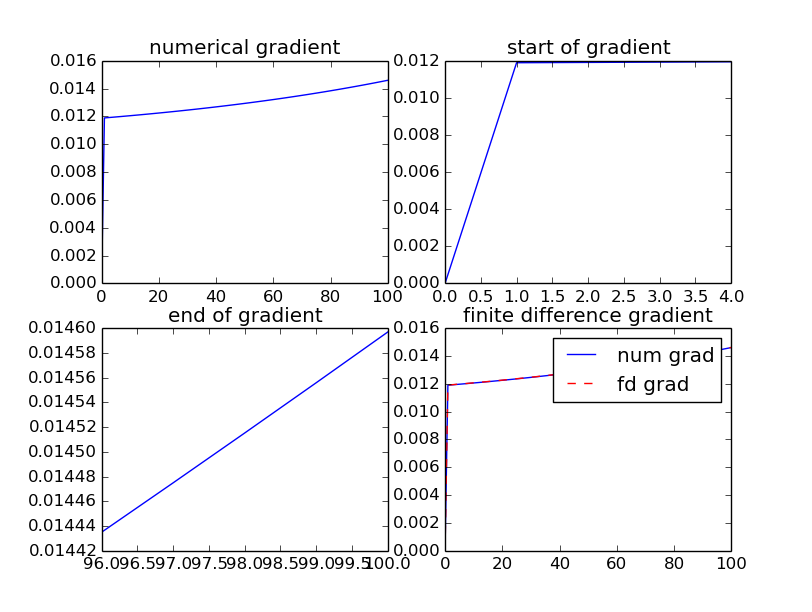
\includegraphics[scale=0.5]{num_grad.png}
\end{figure}
\subsection{Verifying the penalized numerical gradient using the Taylor test}
We will now use the Taylor test on the penalized numerical gradient (\ref{num_pen_grad_lam}-\ref{num_pen_grad_v}) that we get when decomposing $I=[0,T]$ into $N=10$ subintervals while solving the following problem:
\begin{align}
&J(y,v) = \frac{1}{2}\int_0^1v(t)^2dt + \frac{1}{2}(y(1)-1.5)^2\\
&\left\{
     \begin{array}{lr}
       	y'(t)=0.9y(t) +v(t), \ t \in (0,1)\\
       	   y(0)=3.2
     \end{array}
   \right. 
\end{align}
We then discretize in time using $\Delta t=\frac{1}{100}$. The control variable is now a vector $v\in\mathbb{R}^{N+m}$ and we set $v_k=0 \ \forall k=0,...,N+n-1$, while the $w_k$s are chosen randomly from numbers between 0 and 100. Applying the Taylor test to this problem, and letting $D_1$ and $D_2$ be defined as in (\ref{D1}-\ref{D2}) yielded the following:
\\
\begin{table}[!h]
\caption{Taylor test}
\centering
\label{Taylor_tab2}
\begin{tabular}{lrrrll}
\toprule
{}$\epsilon$&  $D_1$ &  $D_2$ &        $||\epsilon w||_{l_{\infty}}$ &    $ \log(\frac{D_1(10\epsilon)}{D_1(\epsilon)})$ &    $ \log(\frac{D_2(10\epsilon)}{D_2(\epsilon)})$  \\
\midrule
1.000000e+00 &  1.080513e+04 &        1.076907e+04 &  9.771288e+01 &       -- &       -- \\
1.000000e-01 &  1.112972e+02 &        1.076907e+02 &  9.771288e+00 &  1.98715 &        2 \\
1.000000e-02 &  1.437558e+00 &        1.076907e+00 &  9.771288e-01 &  1.88886 &        2 \\
1.000000e-03 &  4.683423e-02 &        1.076907e-02 &  9.771288e-02 &  1.48706 &        2 \\
1.000000e-04 &  3.714207e-03 &        1.076907e-04 &  9.771288e-03 &   1.1007 &        2 \\
1.000000e-05 &  3.617285e-04 &        1.076907e-06 &  9.771288e-04 &  1.01148 &        2 \\
1.000000e-06 &  3.607593e-05 &        1.076908e-08 &  9.771288e-05 &  1.00117 &        2 \\
1.000000e-07 &  3.606624e-06 &        1.076979e-10 &  9.771288e-06 &  1.00012 &  1.99997 \\
1.000000e-08 &  3.606527e-07 &        1.086074e-12 &  9.771288e-07 &  1.00001 &  1.99635 \\
\bottomrule
\end{tabular}
\end{table}
\\
\\
Again we see that $|J(v+\epsilon w)-J(v)-\epsilon \nabla J(v)\cdot w|$ converges to zero at a second order rate, meaning that the penalized numerical gradient also passes the Taylor test.
\begin{figure}[h]
\caption{Plots showing the $\Lambda$ and control part of the numerical gradient found using formula (\ref{num_pen_grad_lam}-\ref{num_pen_grad_v}) and finite difference}
\centering
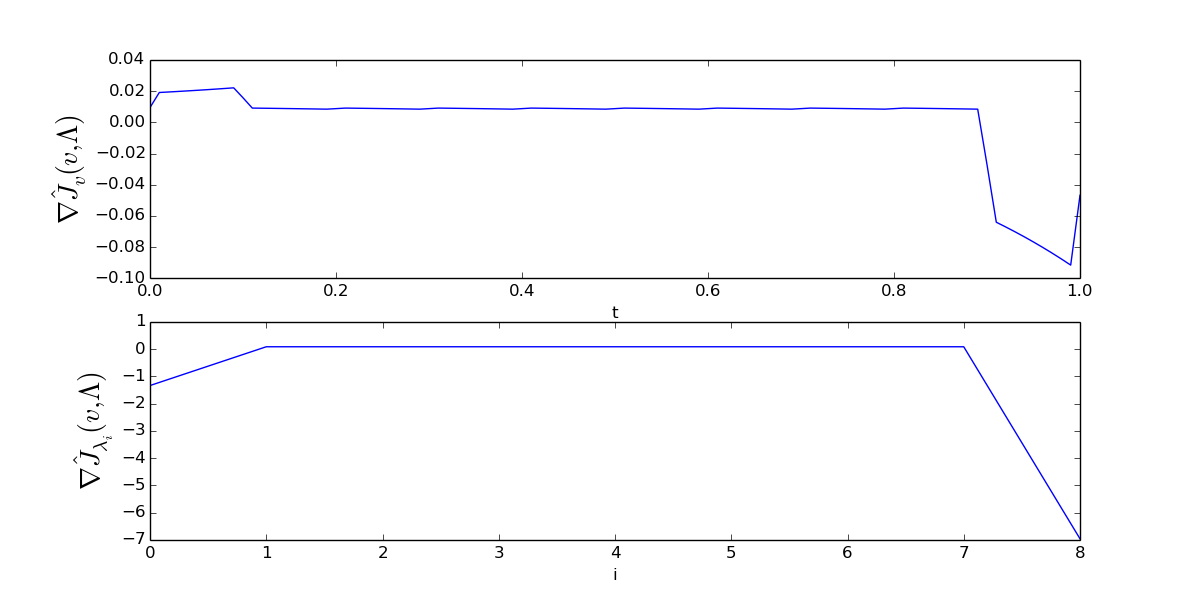
\includegraphics[scale=0.5]{pen_num_grad.png}
\end{figure}
\section{Verifying function and gradient evaluation speedups} \label{ver S sec}
In \ref{analysis sec} we derived the theoretical speedup for numerical gradient and objective function evaluation when decomposing the time-interval. It would now be interesting to check if the implementation achieves the theoretical speedup for our example problem. The specific problem is:
\begin{align*}
&J(y,v) = \frac{1}{2}\int_0^1v(t)^2dt + \frac{1}{2}(y(T)-1)^2 \\
&\left\{
     \begin{array}{lr}
       	y'(t)+y(t) = v(t) \ t\in(0,1)\\
       	y(0)=1
     \end{array}
   \right. 
\end{align*}
A computer with 6 cores was used to verify the results of section \ref{analysis sec}. Having 6 cores means that we can do gradient and function evaluation for $N=1,2,...,6$ decompositions with different time step sizes $\Delta t$. For each combination of $N$ and $\Delta t$, we will run the function and gradient evaluations ten times, and then choose the the smallest execution time produced by the ten runs. The speedup is then calculated by dividing the sequential execution time by the parallel execution time. Below follows tables showing runtime and speedup for both gradient and function evaluation for different $\Delta t$s and $N$s. All evaluations are done with control input $v=1$ and $\lambda_i=1$.  
\\
\begin{table}[!h]
\centering
\caption{$\Delta t=10^{-2}$}
\begin{tabular}{lrr}
\toprule
{} $N$&   function speedup &      function time \\
\midrule
1 &  1.000000 &  0.000196 \\
2 &  0.946860 &  0.000207 \\
3 &  0.780876 &  0.000251 \\
4 &  0.642623 &  0.000305 \\
5 &  0.544444 &  0.000360 \\
6 &  0.427948 &  0.000458 \\
\bottomrule
\end{tabular}
\begin{tabular}{lrr}
\toprule
{} &  gradient speedup &     gradient time \\
\midrule
1 &  1.000000 &  0.000217 \\
2 &  0.875000 &  0.000248 \\
3 &  0.753472 &  0.000288 \\
4 &  0.632653 &  0.000343 \\
5 &  0.547980 &  0.000396 \\
6 &  0.480088 &  0.000452 \\
\bottomrule
\end{tabular}
\end{table}
\begin{table}[!h]
\centering
\caption{$\Delta t=10^{-4}$}
\begin{tabular}{lrr}
\toprule
{} $N$&  function speedup &    function  time \\
\midrule
1 &  1.000000 &  0.008877 \\
2 &  1.983687 &  0.004475 \\
3 &  2.838823 &  0.003127 \\
4 &  3.582324 &  0.002478 \\
5 &  4.267788 &  0.002080 \\
6 &  4.519857 &  0.001964 \\
\bottomrule
\end{tabular}
\begin{tabular}{lrr}
\toprule
{} &  gradient speedup &     gradient time \\
\midrule
1 &  1.000000 &  0.015016 \\
2 &  1.946843 &  0.007713 \\
3 &  2.816204 &  0.005332 \\
4 &  3.677688 &  0.004083 \\
5 &  4.457109 &  0.003369 \\
6 &  4.978780 &  0.003016 \\
\bottomrule
\end{tabular}
\end{table}
\begin{table}[!h]
\centering
\caption{$\Delta t=10^{-5}$}
\begin{tabular}{lrr}
\toprule
{}$N$ &  function speedup &    function  time \\
\midrule
1 &  1.000000 &  0.087484 \\
2 &  2.006606 &  0.043598 \\
3 &  2.888595 &  0.030286 \\
4 &  3.913222 &  0.022356 \\
5 &  4.848102 &  0.018045 \\
6 &  5.425028 &  0.016126 \\
\bottomrule
\end{tabular}
\begin{tabular}{lrr}
\toprule
{} &  gradient speedup &     gradient time \\
\midrule
1 &  1.000000 &  0.154841 \\
2 &  2.046537 &  0.075660 \\
3 &  2.971198 &  0.052114 \\
4 &  4.003025 &  0.038681 \\
5 &  4.921368 &  0.031463 \\
6 &  5.755101 &  0.026905 \\
\bottomrule
\end{tabular}
\end{table}
\begin{table}[!h]
\centering
\caption{$\Delta t=10^{-7}$}
\begin{tabular}{lrr}
\toprule
{}$N$ &  function speedup &      time \\
\midrule
1 &  1.000000 &  8.350907 \\
2 &  1.987960 &  4.200743 \\
3 &  2.847662 &  2.932549 \\
4 &  3.812545 &  2.190376 \\
5 &  4.647839 &  1.796729 \\
6 &  5.479447 &  1.524042 \\
\bottomrule
\end{tabular}
\begin{tabular}{lrr}
\toprule
{} &  gradient speedup &     gradient  time \\
\midrule
1 &  1.000000 &  14.930247 \\
2 &  2.064043 &   7.233497 \\
3 &  2.966254 &   5.033368 \\
4 &  3.866428 &   3.861509 \\
5 &  4.833081 &   3.089178 \\
6 &  5.744552 &   2.599027 \\
\bottomrule
\end{tabular}
\end{table}
\\
\\
Since the parallel algorithm has some overhead, we do not expect any improvements for small problems. This is reflected in the above results, where we for $\Delta t = 10^{-2}$ see an increased execution time when running function and gradient evaluation in parallel. For $\Delta t = 10^{-4}$ we see only a modest speedup, that is significantly lower than the expected speedup from section \ref{analysis sec}. For $\Delta t \leq 10^{-5}$, however we see speedup results in line with what we expect from the theory.  
\section{Consistency}
When we introduced the penalty method in section \ref{penalty_sec}, we also presented a result showing that the iterates $\{v^k\}$ stemming from the penalty algorithmic framework converged towards the solution of the non-penalized problem $v$. We can write this up as:
\begin{align*}
\lim_{k\rightarrow\infty} v^k = v 
\end{align*}  
An alternative way of looking at this, is to let $v^{\mu}$ be the minimizer of $\hat J_{\mu}$, and instead write the above limit as:
\begin{align}
\lim_{\mu\rightarrow\infty} v^{\mu} = v \label{mu con}
\end{align}
The interpretation of the above limit, is that solving the penalized problem with an ever increasing penalty parameter $\mu$ should result in a solution that is getting closer and closer to the solution of the non-penalized problem. This means that the penalty algorithm is consistent, since it produces the same solution as the ordinary non-decomposed problem. It is therefore worth checking if the implementation of the penalized problem actually has the property (\ref{mu con}). The particular problem, that we will do the consistency test on, is: 
\begin{align}
&J(y,v) = \frac{1}{2}\int_0^1v(t)^2dt + \frac{1}{2}(y(T)-1.5)^2 \label{con J} \\
&\left\{
     \begin{array}{lr}
       	y'(t)=0.9y(t) + v(t) \ t\in(0,1)\\
       	y(0)=3.2
     \end{array}
   \right. \label{con E}
\end{align}
Then we set the time step to be $\Delta t = 10^{-2}$ and let $N=2$ be the number of decomposed subintervals. we solved problem (\ref{con J}-\ref{con E}) for increasing $\mu$ values, and looked at different ways to compare the the solutions $v$ and $v^{\mu}$. We compared the function value these controls gave for both the penalized and non-penalized objective function, and the relative difference between $v$ and $v^{\mu}$ in numerical $L^2$-norm. We also looked at the maximal jump difference in the decomposed state equation for each penalized control solution. The results were as follows:
\\
\begin{table}[h]
\centering
\caption{Consistency of penalty method using 2 decompositions}
\label{Cosistency_table}
\begin{tabular}{lrrrr}
\toprule 
{} $\mu$&  $\frac{J(v_{\mu})-J(v)}{J(v)}$ &  $\frac{J_{\mu}(v_{\mu})-J_{\mu}(v)}{J_{\mu}(v)}$ &         $\sup_i\{y_{k_i}^i-y_{k_i}^{i+1}\}$ &    $\frac{||v_{\mu}-v||}{||v||}$ \\
\midrule
1.000000e+02 &      1.156696e-04 &            -6.364173e-03 &  2.592979e-02 &  4.354868e-03 \\
2.000000e+02 &      2.910231e-05 &            -3.192244e-03 &  1.300628e-02 &  2.184385e-03 \\
5.000000e+02 &      4.674259e-06 &            -1.279348e-03 &  5.212496e-03 &  8.754310e-04 \\
1.000000e+03 &      1.170061e-06 &            -6.400835e-04 &  2.607916e-03 &  4.379957e-04 \\
5.000000e+03 &      4.685038e-08 &            -1.280823e-04 &  5.218505e-04 &  8.764416e-05 \\
7.000000e+03 &      2.390506e-08 &            -9.149070e-05 &  3.727640e-04 &  6.260540e-05 \\
2.000000e+04 &      2.928726e-09 &            -3.202365e-05 &  1.304752e-04 &  2.191336e-05 \\
2.000000e+05 &      2.929008e-11 &            -3.202457e-06 &  1.304789e-05 &  2.191569e-06 \\
3.000000e+05 &      1.302587e-11 &            -2.134974e-06 &  8.698604e-06 &  1.461772e-06 \\
4.000000e+05 &      7.331416e-12 &            -1.601231e-06 &  6.523956e-06 &  1.097020e-06 \\
5.000000e+05 &      4.686680e-12 &            -1.280985e-06 &  5.219167e-06 &  8.766907e-07 \\
6.000000e+05 &      3.256551e-12 &            -1.067488e-06 &  4.349307e-06 &  7.307433e-07 \\
1.000000e+06 &      1.171837e-12 &            -6.404931e-07 &  2.609585e-06 &  4.384698e-07 \\
1.000000e+07 &      1.436812e-14 &            -6.404934e-08 &  2.609587e-07 &  4.724119e-08 \\
2.000000e+07 &      7.016988e-15 &            -3.202467e-08 &  1.304793e-07 &  2.669496e-08 \\
1.000000e+08 &      2.338996e-15 &            -6.404934e-09 &  2.609587e-08 &  2.382013e-08 \\
1.000000e+11 &      5.012134e-15 &            -6.400495e-12 &  2.605338e-11 &  2.378564e-08 \\
1.000000e+12 &      4.009707e-15 &            -6.365411e-13 &  2.607248e-12 &  2.378561e-08 \\
1.000000e+13 &      1.002427e-15 &            -6.348703e-14 &  2.646772e-13 &  1.375728e-08 \\
1.000000e+14 &      1.837783e-15 &            -5.346277e-15 &  2.708944e-14 &  1.375728e-08 \\
1.000000e+16 &      2.004854e-15 &             9.355984e-15 &  3.108624e-15 &  1.375728e-08 \\
\bottomrule
\end{tabular}
\end{table}
\\
What we need to note about the results in table \ref{Cosistency_table}, is that while difference in function value and state equation jump approach machine precision, the relative norm difference $\frac{||v_{\mu}-v||}{||v||}$ does not hit machine precision. The explanation of this is that all the terms in our functional are squared, and a difference of $10^{-8}$ is therefore actually quite close to machine precision, when squared. The jump differences are also squared, however the $\mu$ penalty counter balances this for these terms.

